\documentclass[11pt,letterpaper]{article}
\usepackage{graphicx}
\usepackage{blindtext}
\usepackage{geometry}
\usepackage{amsmath}
\usepackage{amssymb}
\usepackage{enumerate}
\usepackage{fancyhdr}


\pagestyle{fancy}
\fancyhf{}
\rhead{\small {© 2022 All Rights Reserved, Aiden Rosenberg}}
\rfoot{Page \thepage}


\title{AP calc Practice FRQs}
\author{Aiden Rosenberg}
\date{April 2022}

\begin{document}

\maketitle
\section{FRQ \#1}
\begin{center}
    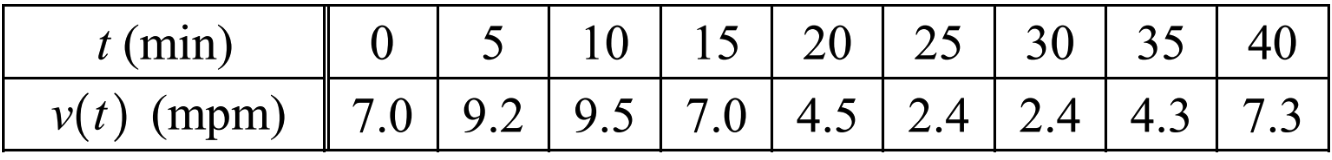
\includegraphics[width=4in]{table7.png}
\end{center}
A test plane flies in a straight line with positive velocity $v(t)$, in miles per minute at time $t$ minutes, where $v$ is a differentiable function of $t$. Selected values of  $v(t)$ for $0\leq t\leq 40 $ are shown in the table above.
\begin{enumerate} [a.)]
    \item Use a midpoint Riemann sum with four subintervals of equal length and values from the table to aproximate $\int_{0}^{40} v(t) \, dt$ Show the computations that lead to your answer. Using correct units, explain the meaning of $\int_{0}^{40} v(t) \, dt$ in terms of the plane’s flight.
    \begin{align*}
        \int_{0}^{40} v(t) \, dt \approx 10 \cdot [9.2+7.0+2.4+4.3] = 229 \, \text {miles}\\
        \text{The plane travels 229 miles during the 40 minutes}.
    \end{align*}
    \item Based on the values in the table, what is the smallest number of instances at which the acceleration of the plane could equal zero on the open interval $0<t<40$? Justify your answer.
    \begin{align*}
        v'(c)=\frac{v(b)-v(a)}{a-b}=0 \, , \text{MVT} \\
        \text{The average rate of change when} \, t\in[25,30] \ \& \ t\in[0,15] \, \text{is zero}.\\
        a \leq c \leq b \therefore \text{There are two possible values where} \, v'(c)=0.
    \end{align*}
    \item The function f, defined by $f(t)=6+\cos(\frac{t}{10})+3\sin(\frac{7t}{40})$  is used to model the velocity of the plane, in miles per minute, for $0\leq t\leq 40$ According to this model, what is the acceleration of the plane at $t = 23$? Indicates units of measure.
    \begin{align*}
        f'(23) \approx -0.407 \, \text {miles per minute}^2
    \end{align*}
    \item According to the model $f$, given in part (c), what is the average velocity of the plane, in miles per minute, over the time interval$0\leq t\leq 40$?
    \begin{align*}
        \frac{1}{40}\int_{0}^{40} f(t) \, dt \approx 5.915 \, \text{miles per minute}
    \end{align*}
\end{enumerate}
\section*{FRQ \#2}
At the beginning of 2010, a landfill contained 1400 tons of solid waste. The increasing function $W$ models
the total amount of solid waste stored at the landfill. Planners estimate that W will satisfy the differential $\frac{dW}{dt}=\frac{1}{25}(W-300)$ equation  for the next 20 years. $W$ is measured in tons, and $t$ is measured in years from the start of 2010. 
\begin{enumerate}[a.)]
    \item Use the line tangent to the graph of $W$ at $t = 0$ to approximate the amount of solid waste that the landfill contains at the end of the first 3 months of 2010 (time $t=\frac{1}{4}$). 
    \begin{align*}
        \frac{dW}{dt}\biggr\rvert_{t=0} = \frac{1}{25}(W(0)-300)=\frac{1}{25}(1400-300)=44\\
        y=44t+1400\biggr\rvert_{t=\frac{1}{4}} = 1411 \, \text{tons}
    \end{align*}
    \item Find $\frac{d^2W}{dt^2}$ in terms of W.  Use $\frac{d^2W}{dt^2}$ to determine whether your answer in part (a) is an underestimate or an overestimate of the amount of solid waste that the landfill contains at time $t=\frac{1}{4}$.
    \begin{align*}
        \frac{d^2W}{dt^2}=\frac{1}{25}\frac{dW}{dt}=\frac{1}{625}(W-300)\biggr\rvert_{W=1400} =1.76.\\
        \text{Since} \frac{d^2W}{dt^2}>0 \, \text{when}\, t\in[0,\frac{1}{4}] \therefore \text{ part (a) is an underestimate}   
    \end{align*}
    \item Find the particular solution $W= W()$ to the differential equation $\frac{dW}{dt}=\frac{1}{25}(W-300)$ with initial condition $W(0)=1400$.
    \begin{align*}
        \frac{dW}{dt}=\frac{1}{25}(W-300) \\
        \int \frac{1}{W-300}\,dW= \int \frac{1}{25}\, dt \\
        \ln |W-300|={1}{25}t+C\\
        \ln|1400-300|=\frac{1}{25}(0)+C \Rightarrow C= \ln|1100|\\
        W-300=1100e^{\frac{1}{25}t}\\
        W(t)=1100e^{\frac{1}{25}t}+300 \, \text{when}\, t \in[0,20]
    \end{align*}
\end{enumerate}
\section*{FRQ \#3}
 For $0\leq t \leq 31$, the rate of change of the number of mosquitoes on Tropical Island at time $t$ days is modeled by $R(t)=5\sqrt t \cos(\frac{t}{5})$ mosquitoes per day. There are 1000 mosquitoes on Tropical Island at time $t = 0$.
 \begin{enumerate}[a.)]
     \item Show that the number of mosquitoes is increasing at time $t = 6$.
     \begin{align*}
         R(6)\approx 4.437 \because  R(6)>0 \, , \text{the number of mosquitoes is increasing at} \, t=6
     \end{align*}
     \item At time $t = 6$, is the number of mosquitoes increasing at an increasing rate, or is the number of mosquitoes increasing at a decreasing rate? Give a reason for your answer.
     \begin{align*}
         R'(6) \approx -1.913 \Rightarrow  R'(6)<0  \\
         \therefore \text{the number of mosquitoes is increasing at a decreasing rate}.
     \end{align*}
     \item According to the model, how many mosquitoes will be on the island at time $t = 31$? Round your answer to the nearest whole number.
     \begin{align*}
         1000 +\int_{0}^{31} R(t)\, dt \approx 964 \, \text{mosquitoes}
     \end{align*}
     \item  To the nearest whole number, what is the maximum number of mosquitoes for
$0\leq t \leq 31$ Show the analysis that leads to your conclusion.
\begin{align*}
    R(t)=0 \, \text{when} \, t=\{0,2.5\pi,7.5\pi\}\\
    R(t)>0 \, \text{when} \, t\in[0,2.5\pi] \, \& \, t\in[7.5\pi, 31] \\
    R(t)<0 \, \text{when} \, t\in[2.5\pi,7.5\pi]\\
    \text{Absolute max is at the 2.5$\pi$ or at the end points}\\
    1000 +\int_{0}^{2.5\pi} R(t)\, dt \approx 1039 \, \text{mosquitoes} 
\end{align*}
\end{enumerate}
\section*{FRQ \#4}
\begin{center}
    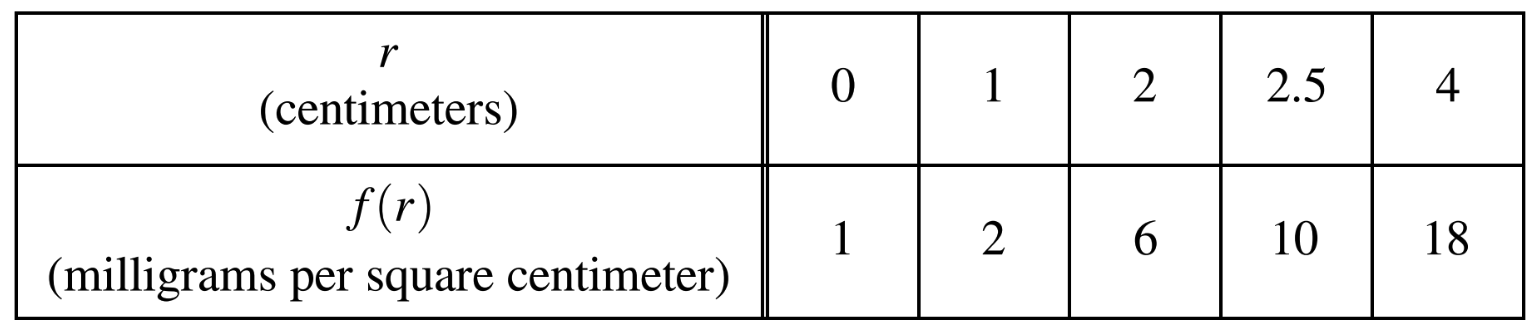
\includegraphics[width=4in]{table3.png}
\end{center}
The density of a bacteria population in a circular petri dish at a distance $r$ centimetres from the centre of the dish is given by an increasing, differentiable function $f$, where $f(r)$ is measured in milligrams per square centimetre. Values of $f(r)$ for selected values of $r$ are given in the table above.
\begin{enumerate} [a.)]
    \item Use the data in the table to estimate $f'(2.25)$. Using correct units, interpret the meaning of your answer in the context of this problem.
    \begin{align*}
        f'(2.25)\approx \frac{f(2.5)-f(2)}{2.5-2}=8 \\
    \end{align*}
At distance $r=2.25$ from the centre of the petri dish, the density of the bacteria population is increasing at a rate of 8 milligrams per square centimetre per centimetre.
\item The total mass, in milligrams, of bacteria in the petri dish is given by the integral expression $2\pi \int_{0}^4 rf(r)\,dr$. Approximate the value of $2\pi \int_{0}^4 rf(r)\,dr$ using a right Riemann sum with the four subintervals indicated by the data in the table.
\begin{align*}
    RHS_{4} & = 2\pi(1\cdot f(1)\cdot(1-0)+2\cdot f(2)\cdot(2-1)+2.5\cdot f(2.5)\cdot(2.5-2)\\+4\cdot f(4)\cdot(4-2.5))\\
     & = 269\pi
    \end{align*}
    \item Is the approximation found in part (b) an overestimate or underestimate of the total mass of bacteria in the petri dish? Explain your reasoning.
    \begin{align*}
        \frac{d}{dr}(r\cdot f(r))=f(r)+r\cdot f'(r)
    \end{align*}
    Since $f'(r)>0$ \& $r > 0$ when $t \in [0,4]$ $ \Longrightarrow \, \frac{d}{dr}(r\cdot f(r)>0$ when $t \in [0,4]$ $\therefore$ the right Riemann sum of $2\pi \int_{0}^4 rf(r)\,dr$ is an overestimate 
    \item The density of bacteria in the petri dish, for $1\leq t \le 1  4$, is modeled by the function $g$ defined by $g(r)=2-16(\cos(1.57\sqrt{r}))^3$. For what value of $k$ , $1<k<1  4$, is $g(k)$ equal to the average value of $g(r)$ on the interval $1\leq k \leq4$?
    \begin{align*}
        g_{avg}=\frac{1}{4-1} \cdot \int_{1}^{4} g(r) \, dr \\
          g_{avg} \approx 9.875\\
          g(k) = g_{avg} \, \Longrightarrow \, k\approx 2.497
    \end{align*}
\end{enumerate}
\section*{FRQ \# 5}
A particle, $P$, is moving along the $x$-axis. The velocity of particle $P$ at time $t$ is given by $v_{P}(t)= \sin(t^{1.5})$ for $0 \leq t\leq \pi$. At time $t = 0$, particle P is at position $x = 5$. A second particle, $Q$, also moves along the $x$-axis. The velocity of particle $Q$ at time $t$ is given by $v_Q(t)=(t-1.8)\cdot 1.25^t$ for $0 \leq t\leq \pi$. At time $t = 0$, particle $Q$ is at position $x = 10$.
\begin{enumerate}[a.)]
    \item Find the positions of particles $P$ and $Q$ at time $t = 1$.
    \begin{align*}
        x_{P}(1)=5+\int_{0}^{1} v_{P}(t) \, dt \approx 5.3706\\
        x_{Q}(1)=10+\int_{0}^{1} v_{Q}(t) \, dt \approx 8.5643\\
    \end{align*}
    \item Are particles $P$ and $Q$ moving toward each other or away from each other at time $t = 1$? Explain your reasoning.
     \begin{align*}
     v_P(1) \approx 0.841471 \because  v_P(1)>0 \, \text{particle $P$ is moving to the right.} \\
     v_Q(1) = -1 \because  v_Q(1)<0 \, \text{particle $Q$ is moving to the left.} \\
    \end{align*}
   At time $t = 1$, $x_P(1)<x_q(1)$ $\therefore$ particle $P$ is to the left of particle $Q$. Hence at time $t = 1$, particles $P$ and $Q$ are moving toward each other.
   \item Find the acceleration of particle $Q$ at time $t = 1$. Is the speed of particle Q increasing or decreasing at time $t = 1$ ? Explain your reasoning.
   \begin{align*}
       v_Q'(1) \approx 1.0268\\
       v_Q(1)=-1
   \end{align*}
$\because$ the velocity of the particle is less than zero and acceleration is greater than zero,at $t=1$; the speed of particle $Q$ is decreasing.
\item Find the total distance travelled by particle P over the time interval $0\leq t \leq\pi$.
\begin{align*}
\int_{0}^{\pi} |v_{P}(t)| \, dt = 1.93148
\end{align*}
\end{enumerate}
\section*{FRQ #5}
\begin{center}
    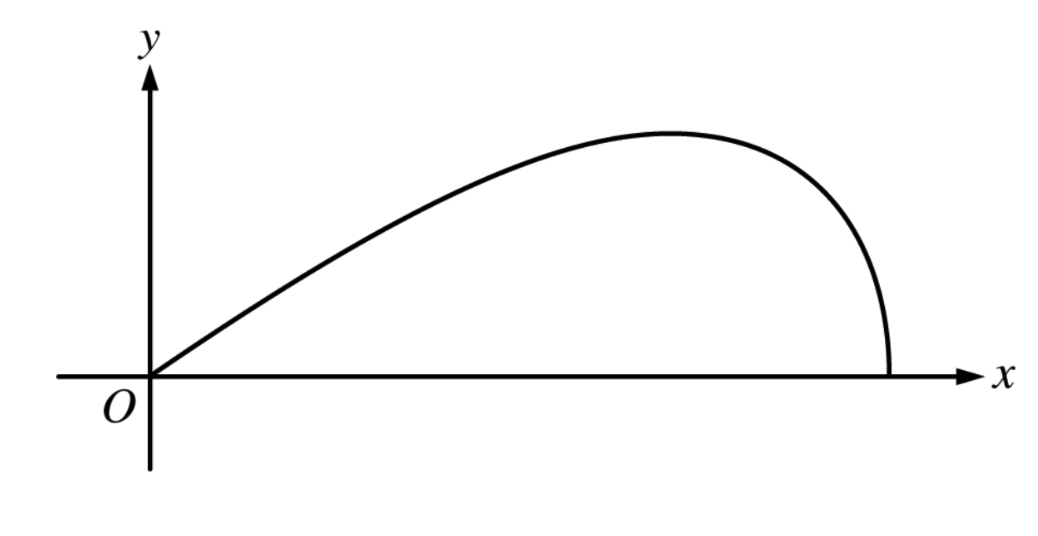
\includegraphics[width=2in]{Graph1.png}
\end{center}
A company designs spinning toys using the family of functions $y=cx\sqrt{4-x^2}$ where $c$ is a positive constant. The figure above shows the region in the first quadrant bounded by the $x$-axis and the graph of $y=cx\sqrt{4-x^2}$ , for some $c$. Each spinning toy is in the shape of the solid generated when such a region is revolved about the $x$-axis. Both $x$ and $y$ are measured in inches.
\begin{enumerate}[a.)]
    \item Find the area of the region in the first quadrant bounded by the $x$-axis and the graph of $y=cx\sqrt{4-x^2}$ for $c = 6$.
    \begin{align*}
       0=6x\sqrt{4-x^2} \Rightarrow x=0, \, x=2\\
        \int_{0}^2 6x\sqrt{4-x^2} \, dx\\
        u=4-x^2 \Rightarrow du=2x \, dx \\
         -3 \int_{4}^0 u^{1/2} \, du \Longrightarrow   3\int_{0}^4 u^{1/2} \, du\\
         = 2u^{3/2} \biggr\rvert_{0}^{4} =2(4^{3/2}) = 16
    \end{align*}
\item It is known that, for $y=cx\sqrt{4-x^2}$, $\frac{dy}{dx}=\frac{c(4-2x^2)}{\sqrt{4-x^2}}$ . For a particular spinning toy, the radius of the largest cross-sectional circular slice is 1.2 inches. What is the value of $c$ for this spinning toy?
\begin{align*}
    0 = \frac{c(4-2x^2)}{\sqrt{4-x^2}} \Rightarrow x=\sqrt{2}\\
    y= c\sqrt{2} \sqrt{4-(\sqrt{2})^2} = c\sqrt{2} \sqrt{2} =2c\\
    1.6=2c \Rightarrow c=0.6
\end{align*}
\newpage
\item For another spinning toy, the volume is $2\pi$ cubic inches. What is the value of $c$ for this spinning toy?
\begin{align*}
    2\pi= \pi\int_{0}^{2} (cx\sqrt{4-x^2})^2 \, dx\\
    2=c^2\int_{0}^{2} x^2(4-x^2))^2\\
    2=c^2\int_{0}^{2} (4x^2-x^4)\\
    2=c^2 \left[ \frac{4}{3}x^3 -\frac{x^5}{5} \right]_{0}^{2} \\ 
    2=c^2 \cdot\frac{64}{15} \\
    c= \sqrt{\frac{15}{32}}
\end{align*}
\end{enumerate}
\newpage
\section*{FRQ \#6}
\begin{center}
    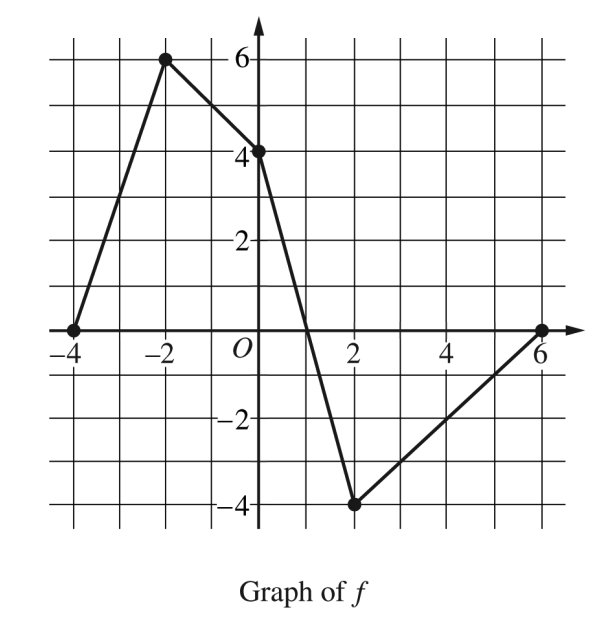
\includegraphics[width=2.5in]{GraphG.png}
\end{center}
Let $f$ be a continuous function defined on the closed interval $−4 \leq x \leq 6$. The graph of $f$, consisting of four line segments, is shown above. Let $G$ be the function defined by $G(x)=\int_{0}^{x} f(t) \, dt$.
\begin{enumerate}
    \item On what open intervals is the graph of $G$ concave up? Give a reason for your answer.
    \begin{align*}
        G'(x)=f(x) \Longrightarrow G''(x)=f'(x)\\
       f'(x) >0 \text{ when } x\in[-4,-2] \; \& \; x\in[2,6] \\
      \therefore \text{ G is CCU} \text{ when } x\in[-4,-2] \; \& \; x\in[2,6]
    \end{align*}
    \item Let $P$ be the function defined by $P(x)=g(x)\cdot f(x)$. Find $P'(3)$.
    \begin{align*}
        P'(x)=G'(x)\cdot f(x)+ f'(x)\cdot G(x)\\
        G'(x)=f(x) \; \& \; G(x)=\int_{0}^{x} f(t) \, dt\\
        \Rightarrow P'(3)=f(3)\cdot f(3)+ f'(3)\cdot \int_{0}^{3} f(t) \, dt\\
        \Rightarrow (-3)(-3)+(1)(\frac{-7}{2})=\frac{11}{2}
    \end{align*}
    \item Find $\lim_{x\to2} \frac{G(x)}{x^2-2x}$
    \begin{align*}
        G(2)=\int_{0}^{2} f(t) \, dt =0 \\
        (2)^2-2(2)=0 \\
        \lim_{x\to2} \frac{G(x)}{x^2-2x} \overset{\mathrm{H}}{=}\\
          \lim_{x\to2} \frac{G(x)}{x^2-2x} =   \lim_{x\to2} \frac{G'(x)}{2x-2} = \frac{-4}{2}=-2
    \end{align*}
    \item Find the average rate of change of $G$ on the interval $[−4, 2]$. Does the Mean Value Theorem guarantee a value $c$, $−4 < c < 2$, for which $G'(c)$ is equal to this average rate of change? Justify your answer.
    \begin{align*}
G(2)=\int_{0}^{2} f(t) \, dt =0 \; \& \; G(-4)=\int_{0}^{-4} f(t) \, dt =-16 \\
\frac{G(2)-G(-4)}{2-(-4)} =\frac{16}{6}= \frac{8}{3}
    \end{align*}
Yes, $G'(x)=f(x) \because G$ is differentiable when $x\in(-4,2) \therefore G$ & continuous when $x\in[-4,2]$ ergo MVT applies. This guarantees for $-4 < c < 2$ $f'(c)=\frac{8}{3}$.
\end{enumerate}
\section*{FRQ \# 7}
Consider the function $y = f(x)$ whose curve is given by the equation $2y^2-6 = y \sin x$ for $y > 0$.
\begin{enumerate}[a.)]
    \item Show that $\frac{dy}{dx}=\frac{y\cos x}{4y-\sin x}$
    \begin{align*}
        4y\frac{dy}{dx}=\frac{dy}{dx} \cdot \sin x + y\cos x\\
        4y\frac{dy}{dx}-\frac{dy}{dx} \cdot \sin x = y\cos x\\
        \frac{dy}{dx}(4y-\sin x) = y\cos x\\
        \frac{dy}{dx} = \frac{y\cos x}{4y-\sin x}
    \end{align*}
    \newpage
    \item Write an equation for the line tangent to the curve at the point $(0, \sqrt{3})$.
    \begin{align*}
        \frac{dy}{dx} =\frac{y\cos x}{4y-\sin x} \biggr\rvert_{(0, \sqrt{3})} = \frac{1}{4}\\
        y=\frac{1}{4}x+\sqrt{3}
    \end{align*}
    \item For $0 \leq x  \leq \pi $ and $y > 0$, find the coordinates of the point where the line tangent to the curve is horizontal.
    \begin{align*}
        \frac{y\cos x}{4y-\sin x}=0 \\ 
        0=y\cos x \Rightarrow x=\frac{\pi}{2}\\
        2y^2-6=y\sin(\frac{\pi}{2})\\
         2y^2-6=y \\
         0=2y^2-6-y\\
         0=(2y+3)(y-2)
    \end{align*}
     Since $4(2)-\sin(\frac{\pi}{2})\neq0 \therefore$ at $(\frac{\pi}{2}, 2)$ the line tangent to the curve is horizontal.
     \item Determine whether $f$ has a relative minimum, a relative maximum, or neither at the point found in part (c). Justify your answer.
     \begin{align*}
         \frac{d^2y}{dx^2}=\frac{(\frac{dy}{dx} \cos x -y\sin x)(4y-\sin x)-(4x\frac{dy}{dx}-\cos x)(y\cos x)}{(4y-\sin x)^2}\\
        \frac{d^2y}{dx^2}\biggr\rvert_{(\frac{\pi}{2}, 2)} = \frac{(-2)(8-1)-0}{(8-1)^2}=\frac{-14}{49}=\frac{-2}{7}
     \end{align*}
     $f$ has a relative maximum at $(\frac{\pi}{2}, 2) \because \frac{dy}{dx}=0 \; \& \; \frac{d^2y}{dx^2}<0$. 
\end{enumerate}
\newpage
\section*{FRQ \#8}
A medication is administered to a patient. The amount, in milligrams, of the medication in the patient at time $t$ hours is modeled by a function $y=A(t)$ that satisfies the differential equation $\frac{dy}{dt}=\frac{12-y}{3}$ . At time $t = 0$ hours, there are $0$ milligrams of the medication in the patient.
\begin{enumerate}[a.)]
    \item A portion of the slope field for the differential equation $\frac{dy}{dt}=\frac{12-y}{3}$ is given below. Sketch the solution curve through the point (0, 0).
    \begin{center}
        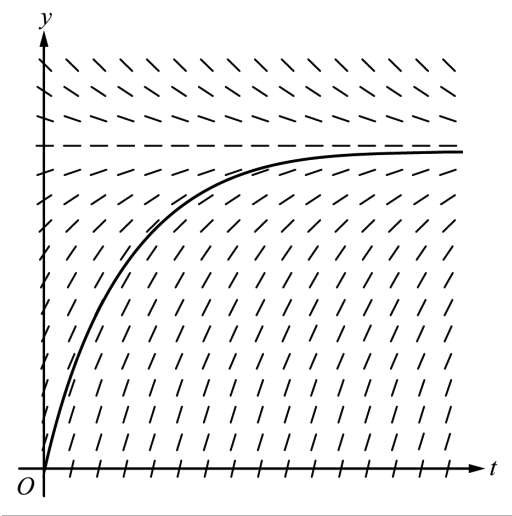
\includegraphics[width=2in]{Slope.png}
    \end{center}
    \item Using correct units, interpret the statement $\lim_{t\to\infty} A(t)=12
$ in the context of this problem.

The amount of medication in the patients blood stream stabilise at $12$ milligrams. 
\item Use separation of variables to find $y = A(t)$, the particular solution to the differential equation $\frac{dy}{dt}=\frac{12-y}{3}$ with initial condition $A(0) = 0$.
\begin{align*}
    \frac{dy}{dt}=\frac{12-y}{3} \Longrightarrow \frac{1}{3} \cdot dy= \frac{1}{(12-y)} \cdot dt \\
    \int \frac{1}{3} \, dt = \int \frac{1}{(12-y)} \, dy \\
    \frac{1}{3}t +C=-\ln(12-y) \\
    C=-\ln(12) \\ 
      -\frac{1}{3}t +\ln(12)=\ln(12-y) \\
      e^{ -\frac{1}{3}t +\ln(12)}=12-y\\
      12 e^{ -\frac{1}{3}t}=12-y\\
       -12 e^{ -\frac{t}{3}}=y
\end{align*}
\item A different procedure is used to administer the medication to a second patient. The amount, in milligrams, of the medication in the second patient at time $t$ hours is modelled by a function $y = B(t$) that satisfies the differential equation $\frac{dy}{dt}= 3-\frac{y}{t+2}$. At time $t = 1$ hour, there are 2.5 milligrams of the medication in
the second patient. Is the rate of change of the amount of medication in the second patient increasing or decreasing at time $t = 1$ ? Give a reason for your answer.
\begin{align*}
    \frac{dy}{dt}\biggr\rvert_{(1,2.5)} =3-\frac{2.5}{3} = \frac{6.5}{3}\\
    \frac{d^2y}{dt^2}= \frac{-\frac{dy}{dt}(t+2)-y}{(t+2)^2} \biggr\rvert_{(1,2.5)} = \frac{-6.5-2.5}{9} =\frac{-4}{9}<0
\end{align*}
Since at $(1,2.5)$ $\frac{d^2y}{dt^2}<0$ and $\frac{dy}{dt}>0$, the amount of medication in the persons blood is increasing at a decreasing rate. 
\end{enumerate}
\end{document}
